\documentclass[tikz, convert = false]{standalone}%

\usepackage[utf8]{inputenx}%  http://ctan.org/pkg/inputenx
% Euler for math | Palatino for rm | Helvetica for ss | Courier for tt
\renewcommand{\rmdefault}{ppl}% rm
\linespread{1.05}% Palatino needs more leading
\usepackage[scaled]{helvet}% ss //  http://ctan.org/pkg/helvet
\usepackage{courier}% tt // http://ctan.org/pkg/courier
\usepackage{eulervm}  %  http://ctan.org/pkg/eulervm
% a better implementation of the euler package (not in gwTeX)
\normalfont%
\usepackage[T1]{fontenc}%  http://ctan.org/pkg/fontenc
\usepackage{textcomp}%  http://ctan.org/pkg/textcomp

\usetikzlibrary{patterns}
\usetikzlibrary{decorations.pathmorphing}

\begin{document}
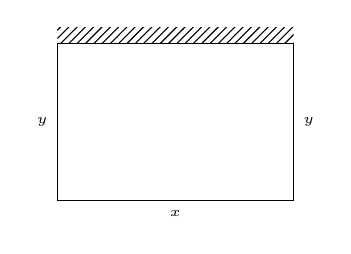
\begin{tikzpicture}
  \fill[pattern = north east lines] (0, 0) rectangle (3, 0.2);

  \draw (0, 0) rectangle (3, -2);

  \node[font = \tiny, right] at (3, -1) {$y$};
  \node[font = \tiny, left] at (0, -1) {$y$};
  \node[font = \tiny, below] at (1.5, -2) {$x$};
\end{tikzpicture}
\end{document}
%%% Local Variables:
%%% mode: latex
%%% TeX-master: t
%%% End: